\documentclass{article}
\usepackage{graphicx}
\usepackage{amsmath}
\usepackage{amssymb}
\usepackage[a4paper, top=25mm, bottom=25mm, left=25mm, right=25mm]{geometry}
\usepackage{pgfplots}
\pgfplotsset{compat=1.18}
\usepackage{mathtools}
\DeclarePairedDelimiter\ceil{\lceil}{\rceil}
\DeclarePairedDelimiter\floor{\lfloor}{\rfloor}

\begin{document}
\large

\begin{center}
2015-2016 Fall Semester\\MAT123-07 Midterm\\(10/12/2015)
\end{center}

\noindent 1) Find all local extrema and inflection points of the function $f(x) = \frac{1}{x} + \frac{1}{x^2}$. On which intervals is the function increasing, decreasing, concave upward, or concave downward? Find all asymptotes. Graph the function.


\hfill

\noindent 2) Use Rolle's theorem to show that $3\tan x + x^3 = 2$ has exactly one solution on the interval $[0,\pi/4]$.

\hfill

\noindent 3) Find the tangent line to the graph of the equation $x \sin(xy-y^2) = x^2-1$, at $(1,1)$.

\hfill

\noindent 4) Evaluate the limits

a. $\displaystyle \lim_{x\to 0^+} (1+\sin x)^{\frac{1}{x}}$

b. $\displaystyle \lim_{x\to 3} \frac{x^2-\floor{x^2}}{x-3}$

\hfill

\noindent 5) A point P is moving in the $xy$-plane. When P is at $(4, 3)$, its distance to the origin is increasing at a rate of $\sqrt{2}$ cm/s, and its distance to the point $(7, 0)$ is decreasing at a rate of 3 cm/s. Determine the rate of change of the $x$-coordinate of P at that moment.

\hfill

\noindent 6) Sketch the region bounded by $y=2|x|$ and $y=8-x^2$. Find the area of the region.

\newpage

\begin{center}
Solutions (Last update: 7/12/25 (12th of July) 5:35 PM)
\end{center}

\noindent 1) Take the first derivative and set to 0.

\begin{equation*}f'(x) = -\frac{1}{x^2} - \frac{2}{x^3}\end{equation*}

\begin{equation*}f'(x) = 0\,\rightarrow\,\frac{2}{x^3} = -\frac{1}{x^2}\,\rightarrow\,x = -2 \, (\text{candidate for a critical point})\end{equation*}

\hfill

\noindent Take the second derivative and set to 0.

\begin{equation*}f''(x) = \frac{2}{x^3} + \frac{6}{x^4}\end{equation*}

\begin{equation*}f''(x) = 0\,\rightarrow\,\frac{1}{x^3} = -\frac{3}{x^4}\,\rightarrow\,x = -3\, (\text{candidate for an inflection point})\end{equation*}

\hfill

\noindent  $\{-2, -3\} \in D$. Therefore, $f(-2)$ gives rise to a local extremum. The sign of the first derivative changes from minus to plus, meaning $f(-2)$ is a local minimum. $x=-3$ gives rise to an inflection point because the sign of the second derivative also changes.

\hfill

\noindent Find the asymptotes.

\begin{equation*}\lim_{x\to\infty} f(x) = \lim_{x\to-\infty} f(x) = 0\end{equation*}

\hfill

\noindent $y=0$ is the horizontal asymptote and $x=0$ is the vertical asymptote.

\hfill

\noindent Let us find monotonicity and concavity. If the sign of $f'(x)$ is minus, the function is decreasing on the corresponding interval; otherwise, increasing. If the sign of $f''(x)$ is minus, the graph of the function is concave downward; otherwise, concave upward.

\begin{center}
    \large
    \begin{tabular}{ |c| c c c c| } 
    \hline
        $x$ & $(-\infty, -3)$ & $(-3, -2)$ & $(-2, 0)$ &  $(0, \infty)$ \\
        \hline
        $f'$ sign & - & - & + & - \\
        \hline
        $f''$ sign & - & + & + & + \\
        \hline
    \end{tabular}
\end{center}

\hfill

\noindent Eventually, sketch the graph.

\begin{center}
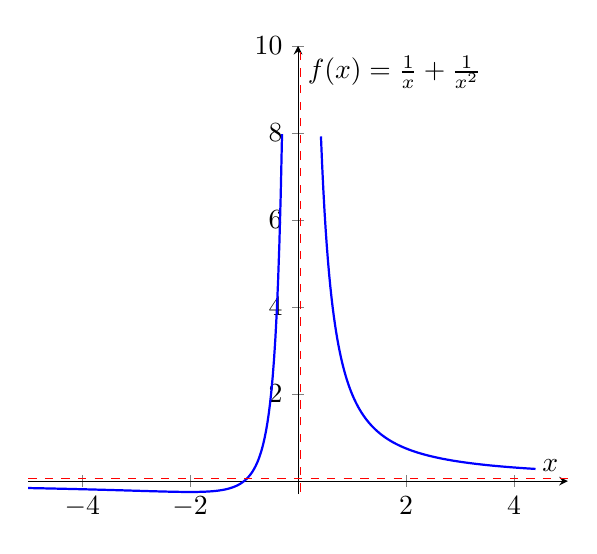
\begin{tikzpicture}
  \begin{axis}[
    axis lines = center,
    xlabel = $x$,
    ylabel = {$f(x) = \frac{1}{x} + \frac{1}{x^2}$},
    domain=-3:-0.1, % left branch
    samples=200,
    ymin=-0.3, ymax=10,
    xmin=-5, xmax=5,
    restrict y to domain=-1:8,
    restrict x to domain=-5:5,
    legend pos=outer north east,
    clip=true
  ]
    \addplot[blue, thick, domain=-5:-0.1] {1/x + 1/(x^2)};
    \addplot[blue, thick, domain=0.1:4.4] {1/x + 1/(x^2)};

    \draw[dashed, red] (axis cs:-5,0.05) -- (axis cs:5,0.05);
    \draw[dashed, red] (axis cs:0.05,-30) -- (axis cs:0.05,30);
  \end{axis}
\end{tikzpicture}
\end{center}

\hfill

\noindent 2) Let $f(x) = 3\tan x + x^3 -2$. $f$ is continuous on $[0, \pi/4]$ and differentiable on $(0, \pi/4)$. By IVT (Intermediate Value Theorem), there exists at least one point where $f(x) = 0$ because $f(0) = -2$ and $f(\pi/4) = 1 + (\pi/4)^3$. Assume that we have two roots on the interval, so at some point c, $f'(c) = 0$.

\begin{equation*}f'(x) = 3\sec^2x + 3x^2\,\rightarrow\, f'(c) = 3\sec^2c + 3c^2 = 0\,\rightarrow\,\sec^2c =-c^2 \end{equation*}

\hfill

\noindent Since $-c^2 \leq 0$ and $\sec ^2c > 0$, there is no $c$ that satisfies the equation. This contradicts our assumption that we have two roots on the interval. By Rolle's theorem, there is only one root on the interval $[0, \pi/4]$.

\hfill

\noindent 3) Implicitly differentiate both sides.

\begin{equation*}\frac{d}{dx}[x \sin(xy-y^2)] = \frac{d}{dx}(x^2-1) \end{equation*}

\begin{equation*}1\cdot \sin(xy-y^2) + x\cdot\cos(xy-y^2) \cdot \Big[\Big(1\cdot y + x\frac{dy}{dx} \Big) -2y\frac{dy}{dx}\Big]= 2x\end{equation*}

\hfill

\noindent Rearrange the equation to solve for $\frac{dy}{dx}$ through a careful and rigorous attempt.

\begin{equation*} x\cdot\cos(xy-y^2) \cdot \Big[\Big(1\cdot y + x\frac{dy}{dx} \Big) -2y\frac{dy}{dx}\Big]= 2x - \sin(xy-y^2)\end{equation*}

\begin{equation*} y + \frac{dy}{dx}(x-2y)= \frac{2x - \sin(xy-y^2)}{x\cdot\cos(xy-y^2)}\end{equation*}

\begin{equation*} \frac{dy}{dx}(x-2y)= \frac{2x - \sin(xy-y^2)}{x\cdot\cos(xy-y^2)} - y\end{equation*}

\hfill

\begin{equation} \frac{dy}{dx} = \frac{\frac{2x - \sin(xy-y^2)}{x\cdot\cos(xy-y^2)} - y}{(x-2y)}\end{equation}

\hfill

\noindent Calculate $\displaystyle \frac{dy}{dx}\Bigg|_{(1,1)}$ from (1). This will give us the slope of the tangent line.

\begin{equation*}\frac{dy}{dx}\Bigg|_{(1,1)} = -1\end{equation*}

\hfill

\noindent Recall: $y-y_0 = m(x-x_0)$. $m$ is $\displaystyle \frac{dy}{dx}$ at $x=1$. So, the tangent line is:

\begin{equation*} y-1 = -(x-1) \,\rightarrow\, \boxed{y=2-x}\end{equation*}

\hfill

\noindent 4)

\hfill

\noindent a) Let L be the value of the limit. Then, take the logarithm of both sides.

\begin{equation*}L = \lim_{x\to 0^+} (1+\sin x)^{\frac{1}{x}}\end{equation*}

\begin{equation*}\ln(L) = \ln\Big[\lim_{x\to 0^+} (1+\sin x)^{\frac{1}{x}}\Big]\end{equation*}

\hfill

\noindent The expression on the right is continuous for $x>0$. Therefore, we can take the logarithm inside the limit.

\begin{equation*}\ln(L) = \lim_{x\to 0^+} \ln\Big[(1+\sin x)^{\frac{1}{x}}\Big] = \lim_{x\to 0^+} \Big[\frac{\ln(1+\sin x)}{x}\Big] \end{equation*}

\hfill

\noindent If we substitute $x=0$, the limit is in the form $0/0$. L'Hôpital's rule states that we may take the derivatives of both sides of the fraction if there's a $0/0$ indeterminate form. Apply the chain rule accordingly.

\begin{equation*}\lim_{x\to 0^+} \Big[\frac{\ln(1+\sin x)}{x}\Big] \overset{\text{L'H.}}{=} \lim_{x\to 0^+} \Big[\frac{\frac{1}{1+\sin x} \cdot \cos x}{1}\Big] = \lim_{x\to 0^+} \Big[\frac{\cos x}{1+\sin x}\Big] \end{equation*}

\hfill

\noindent The limit can now be evaluated by substituting $x=0$.

\begin{equation*}\lim_{x\to 0^+} \Big[\frac{\cos x}{1+\sin x}\Big] = \frac{\cos 0}{1 + \sin 0 } =1\end{equation*}

\hfill

\noindent Now, $\ln(L) = 1$. Simply, take $L$ out of the logarithm.

\begin{equation*} \boxed{L = \mathrm{e}}\end{equation*}

\hfill

\noindent b) Look at the one-sided limits. Let us first evaluate the limit from the right side. Above and near $x=3$, the floor function will return $9$.

\begin{equation*} \lim_{x\to 3^+} \frac{x^2-\floor{x^2}}{x-3} = \lim_{x\to 3^+}\frac{x^2-9}{x-3} = \lim_{x\to 3^+}\frac{(x-3)(x+3)}{x-3} = \lim_{x\to 3^+}(x+3)= 6\end{equation*}

\hfill

\noindent From the left side, the output is the largest integer less than $9$. Therefore, $\floor{x^2} = 8$.

\begin{equation*} \lim_{x\to 3^-} \frac{x^2-\floor{x^2}}{x-3} = \lim_{x\to 3^-}\frac{x^2-8}{x-3} = -\infty\end{equation*}

\hfill

\noindent The one-sided limits are not equal to each other. Therefore, the limit does not exist.

\hfill

\noindent 5) $x=x(t)$ and $y=y(t)$. The distance between the point P and the origin, and the distance between the point P and the point (7,0) are, respectively, given by:

\begin{equation*}f(t) = \sqrt{(x-0)^2 + (y-0)^2} = \sqrt{x^2+y^2}\end{equation*}

\begin{equation*}g(t) = \sqrt{(x-7)^2 + (y-0)^2} = \sqrt{x^2-14x +49+y^2}\end{equation*}

\hfill

\noindent Take the first derivative with respect to time.

\begin{equation}f'(t) =\frac{1}{2\sqrt{x^2+y^2}}\cdot\Big(2x\frac{dx}{dt} + 2y\frac{dy}{dt}\Big)\end{equation}

\begin{equation}g'(t) =\frac{1}{2\sqrt{x^2-14x +49+y^2}}\cdot\Big((2x-14)\frac{dx}{dt} + 2y\frac{dy}{dt}\Big)\end{equation}

\hfill

\noindent For $t=t_0$, it is given $x(t_0) = 4,\,y(t_0) = 3$ and $f(t_0) = \sqrt{4^2 +3^2} = 5,\,g(t_0) = \sqrt{3^2 + 3^2} = 3\sqrt{2}$. We then obtain a system of two equations by substituting values in (2) and (3):

\begin{equation*}f'(t_0) =\frac{1}{10}\cdot\Big(8\frac{dx}{dt}+6\frac{dy}{dt}\Big) = \sqrt{2} \end{equation*}

\begin{equation*}g'(t_0) =\frac{1}{6\sqrt{2}}\cdot\Big((-6)\frac{dx}{dt} + 6\frac{dy}{dt}\Big) = -3\end{equation*}

\hfill

\noindent Let us simplify the equations.

\begin{equation*}4x'(t_0)+3y'(t_0) = 5\sqrt{2} \end{equation*}
\begin{equation*}-3x'(t_0)+3y'(t_0) = -9\sqrt{2} \end{equation*}

\hfill

\noindent The question asks us to find the change in the $x$-coordinate of P. Therefore, negate the latter equation and solve for $x'(t_0)$.

\begin{equation*} \boxed{x'(t_0) = 2\sqrt{2}} \end{equation*}

\hfill

\noindent The change in the $y$-coordinate is left as a practice for the reader.

\hfill

\noindent 6)

\begin{center}
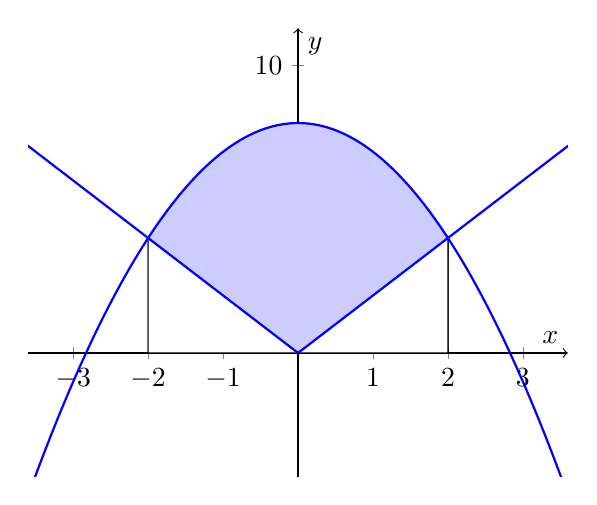
\begin{tikzpicture}
  \begin{axis}[
    axis lines = center,
    xlabel = $x$, ylabel = $y$,
    domain=-4:4,
    samples=300,
    ymin=-3, ymax=10,
    xmin=-3, xmax=3,
    restrict y to domain=-10:10,
    enlargelimits=true,
    legend pos=outer north east,
    axis line style={->},
    ]
    \addplot [
      domain=-2:2,
      samples=200,
      fill=blue!20,
    ]
    {8 - x^2} \closedcycle;

    \addplot [
      domain=-2:2,
      samples=200,
      fill=white,
    ]
    {2*abs(x)} \closedcycle;
    
    \addplot[blue, thick] {2*abs(x)};
    \addplot[blue, thick] {8-x^2};

  \end{axis}
\end{tikzpicture}
\end{center}

\noindent The area can be found by integrating the difference in $y$ with respect to $x$. We split the integral into two because the absolute value function changes sign.

\begin{equation*}\text{I} = \int_{-2}^2 (8-x^2-2|x|)\,dx = \int_{-2}^0 (8-x^2+2x)\,dx + \int_{0}^2 (8-x^2 - 2x)\,dx\end{equation*}

\begin{equation*}\text{I} = \Bigg[8x-\frac{x^3}{3} + x^2 \Bigg]_{-2}^0 + \Bigg[8x-\frac{x^3}{3} - x^2 \Bigg]_{0}^2\end{equation*}

\begin{equation*}\text{I} = 0 - \Big({-16} + \frac{8}{3} + 4\Big) + \Big(16 - \frac{8}{3} - 4\Big) - 0 = \boxed{\frac{56}{3}}\end{equation*}

\end{document}